\label{sec:reco-tracking}
Many algorithms and software designs are available for tracking. For details refer to \cite{newt}. The following presents the reader with a brief summary of major algorithm used by ATLAS as the tracking reconstruction procedure, the so called ``inside-out'' procedure. Track finding starts from the precision detectors pixel and SCT. We first find 3-D representation of pixel and SCT clusters/hits called ``space points''. Then track seed search are done with two pairs ``space points'' with $z$ constraints (tighter cut on the primary vertices) or no constriants (loose cut on primary vertices.) Track seeds at this point contains directional information. The track fitting utilizes Kalman filter following assuming the hit sequence to be a Hidden Markov Model. While the filter moves along the track seeds direction, it incoporates the new hits it sees and updates the track fit with five helix parameters at the perigee of the track. Only 10\% of the seeds evetually lead to real tracks. To resolve the ambiguity arising from seeded tracking, track candidates are ranked by their quality scores. Scores favor tracks with high $\chi^2$, less holes and hits from higher resolution part of the detector. Shared hits are then assigned to higher score tracks and lower score tracks are refitted. For very dense environment, in which the pixel clusters may merge, see for example Fig.\ref{fig:reco-trackingcluster}, neural network tools are utilized to separate apart clusters created by no more than two individual charged particles\cite{PERF-2012-05,PERF-2015-08}. The track segment found by the pixel and SCT collaboratively are then extended to include matched TRT hits. The alignment of the tracker needs to be performed online to reduce hit to track residuals as the thermal condition of the pixel detector changes during data taking. Espeically during the early Run II operation, the IBL was observed to have an unexpected bowing giving rise to an up to 6$\mu m$ vertical shift and needs real time corrections.\cite{tracking-align}.

\begin{figure}[htpb!]
\begin{center}
  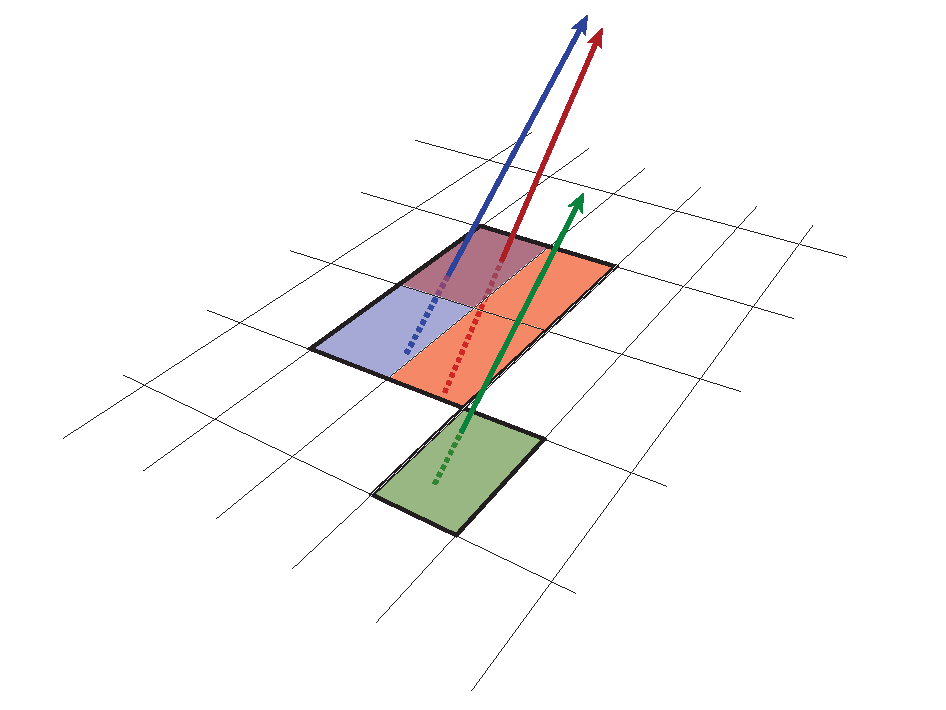
\includegraphics[width=0.55\linewidth]{figures/Reco/TrackingClusterB}
  \caption{ Illustration a merged pixel cluster due to colimated charged particles originating from high energy parent (Ref.\cite{PERF-2015-08}). }
\label{fig:reco-trackingcluster}
\end{center}
\end{figure}


Tracks used by physics analyses need to pass quality and kinematics cuts. The loose track quality is defined as:

\begin{itemize}
\item \pT $>$ 400 \mev
\item $|\eta| < $ 2.5
\item At least 7 silicon (pixel + SCT) hits
\item At most 1 shared modules
\item At most 2 missing silicon hits
\item At most 1 missing pixel hit
\end{itemize}

On top of the criteria of loos tracks, the tight track criteria include also the following:

\begin{itemize}
\item no pixel holes
\item at least on hit on IBL or B-layer
\item silicon hits $\geq$ 9 (if $|\eta|\leq 1.65$)
\item silicon hits $\geq$ 11 (if $|\eta|\geq 1.65$)
\end{itemize}

The reconstruction efficiency of tracks depend on the type of decays, intial particle momentum and psuedo rapidity and so on. Fig. \ref{fig:reco-trackingeff} shows the tracking efficiency as a function of parent particle \pt in different decay modes. Particularly relevant for this thesis the efficiency of tracking for $B$ mesons, which with loose track requirement stays reasonably above 85\% up to 1\TeV. When the pile-up contribution goes up, accidental combinations of hits could also pass all the cuts we apply to the track candidiates and yield so called ``fake'' tracks. This effect is estimated to be $\leq 5\%$ for the loose category tracks with $\mu = 30$ as shown in Fig.\ref{fig:reco-trackingfake}.


\begin{figure}[htpb!]
\begin{center}
  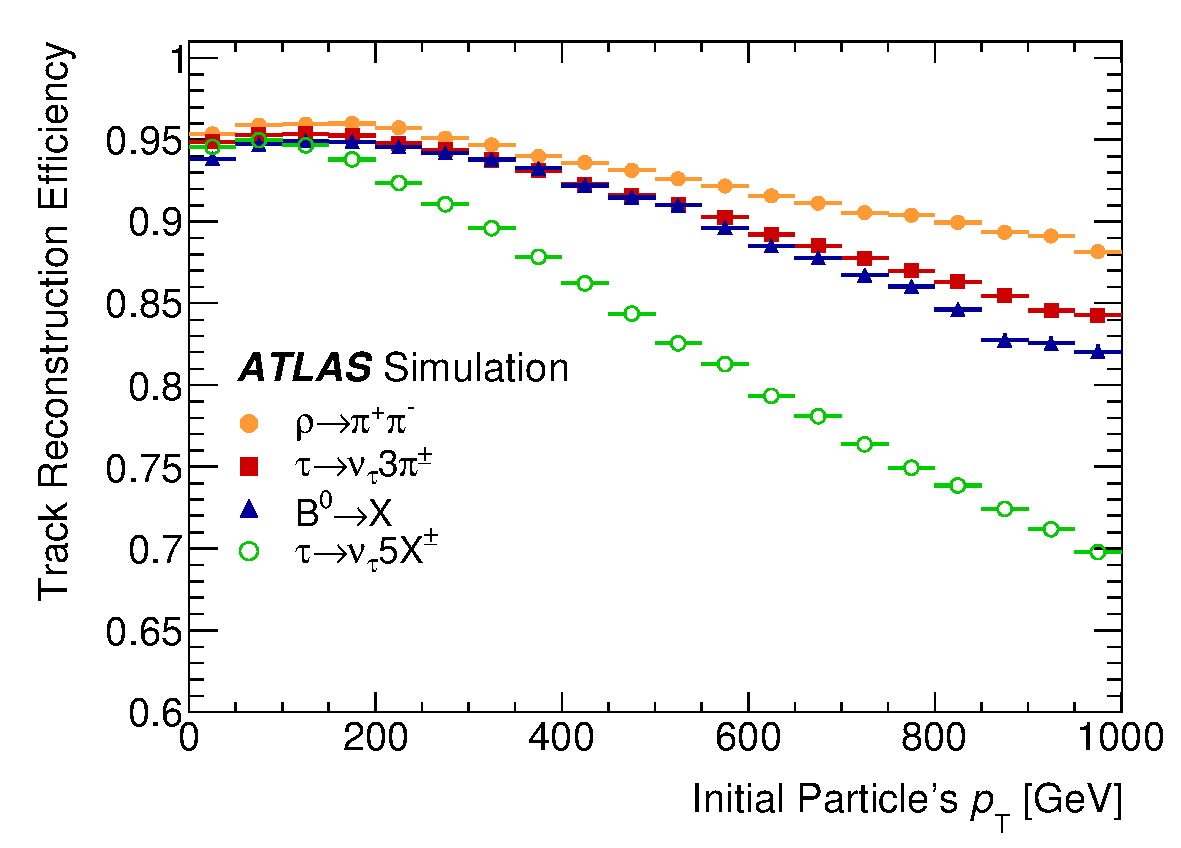
\includegraphics[width=0.55\linewidth]{figures/Reco/TrackingEfficiency}
  \caption{Tracking efficiency as a function of \pt of the parent particle which decays before the IBL for $\rho$, three- and five-prong $\tau$ and B0 (Ref.\cite{PERF-2015-08})}
\label{fig:reco-trackingeff}
\end{center}
\end{figure}

\begin{figure}[htpb!]
\begin{center}
  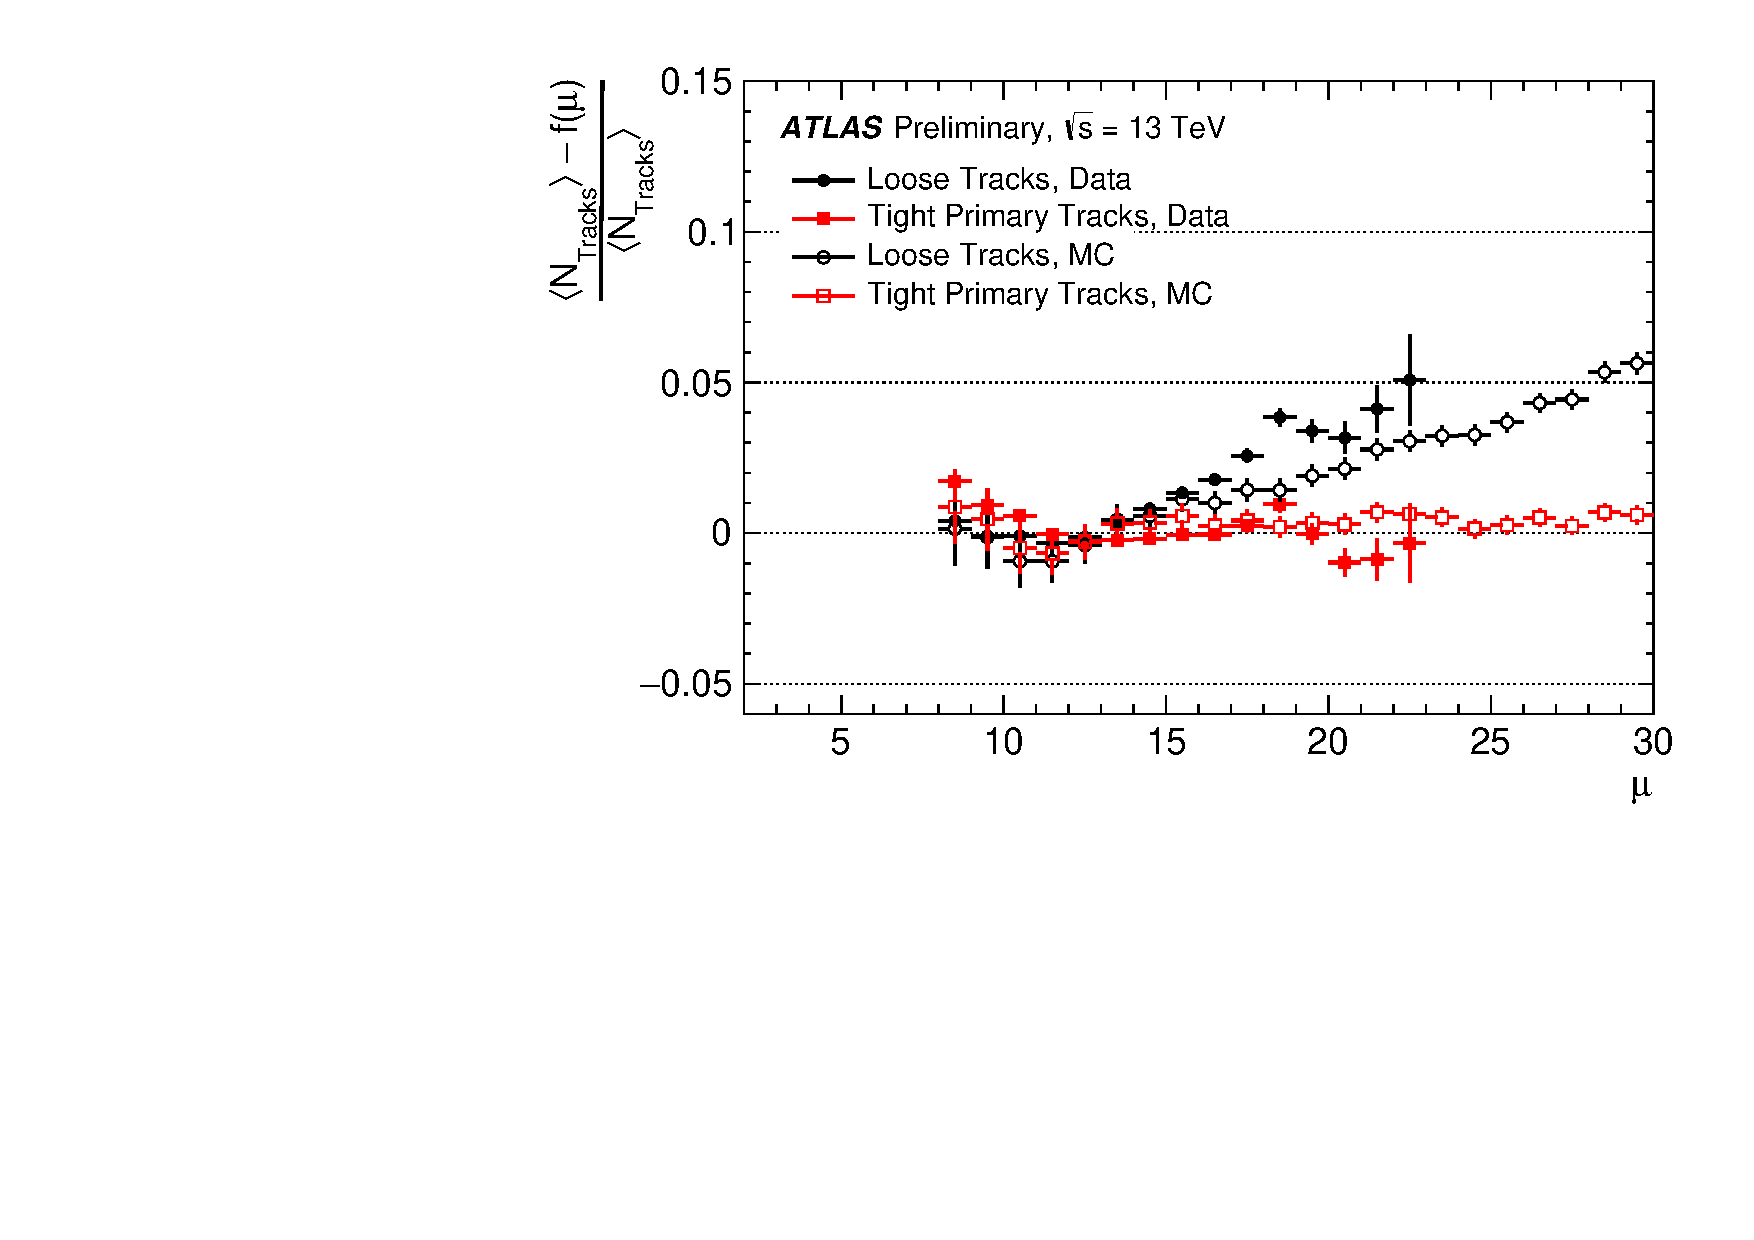
\includegraphics[width=0.55\linewidth]{figures/Reco/TrackingFake}
\caption{An estimation of the tracking fake rate, assuming the real tracks scale linearly as a function of $\mu$ (Ref.\cite{ATL-PHYS-PUB-2015-051}). }
\label{fig:reco-trackingfake}
\end{center}
\end{figure}


The reconstructed tracks can help us find the event primary vertex, where the proton-protn hard scattering takes place. The set of tracks which are considered for vertices finding need to pass:

\begin{itemize}
\item $\pT > 400 \mev$
\item $|d_0|<4mm$, $\sigma(d0) < 5 mm$, $\sigma(z0) < 10 mm$
\item at least 4 SCT hits
\item at least 9 silicon (pixel + SCT) hits
\item no pixel holes
\end{itemize}

The vertices finding algorithm, documented in \cite{PERF-2015-01}, starts with a seed position which is the mode of the z coordinates of all tracks. Knowing the seed, the algorithm iteratively calculates the vertex position by downweighting the tracks which are far away and not compatible with this vertex. Each iteration re-calcualtes the vertex position. Tracks which are 7 $\sigma$ away are considered not belong to this vertex and pooled for the iteration of finding the next vertex. Among all the vertices considered with at least two tracks associated to them, the one with highest track $\sum\pt^2$ is usually deemed as the primary vertex, where the hard-scattering collision event happened. Resolutions of beam spot positions from the fits can usually be improved through the constraints from beam spot positions.

\begin{figure}[htpb!]
\begin{center}
  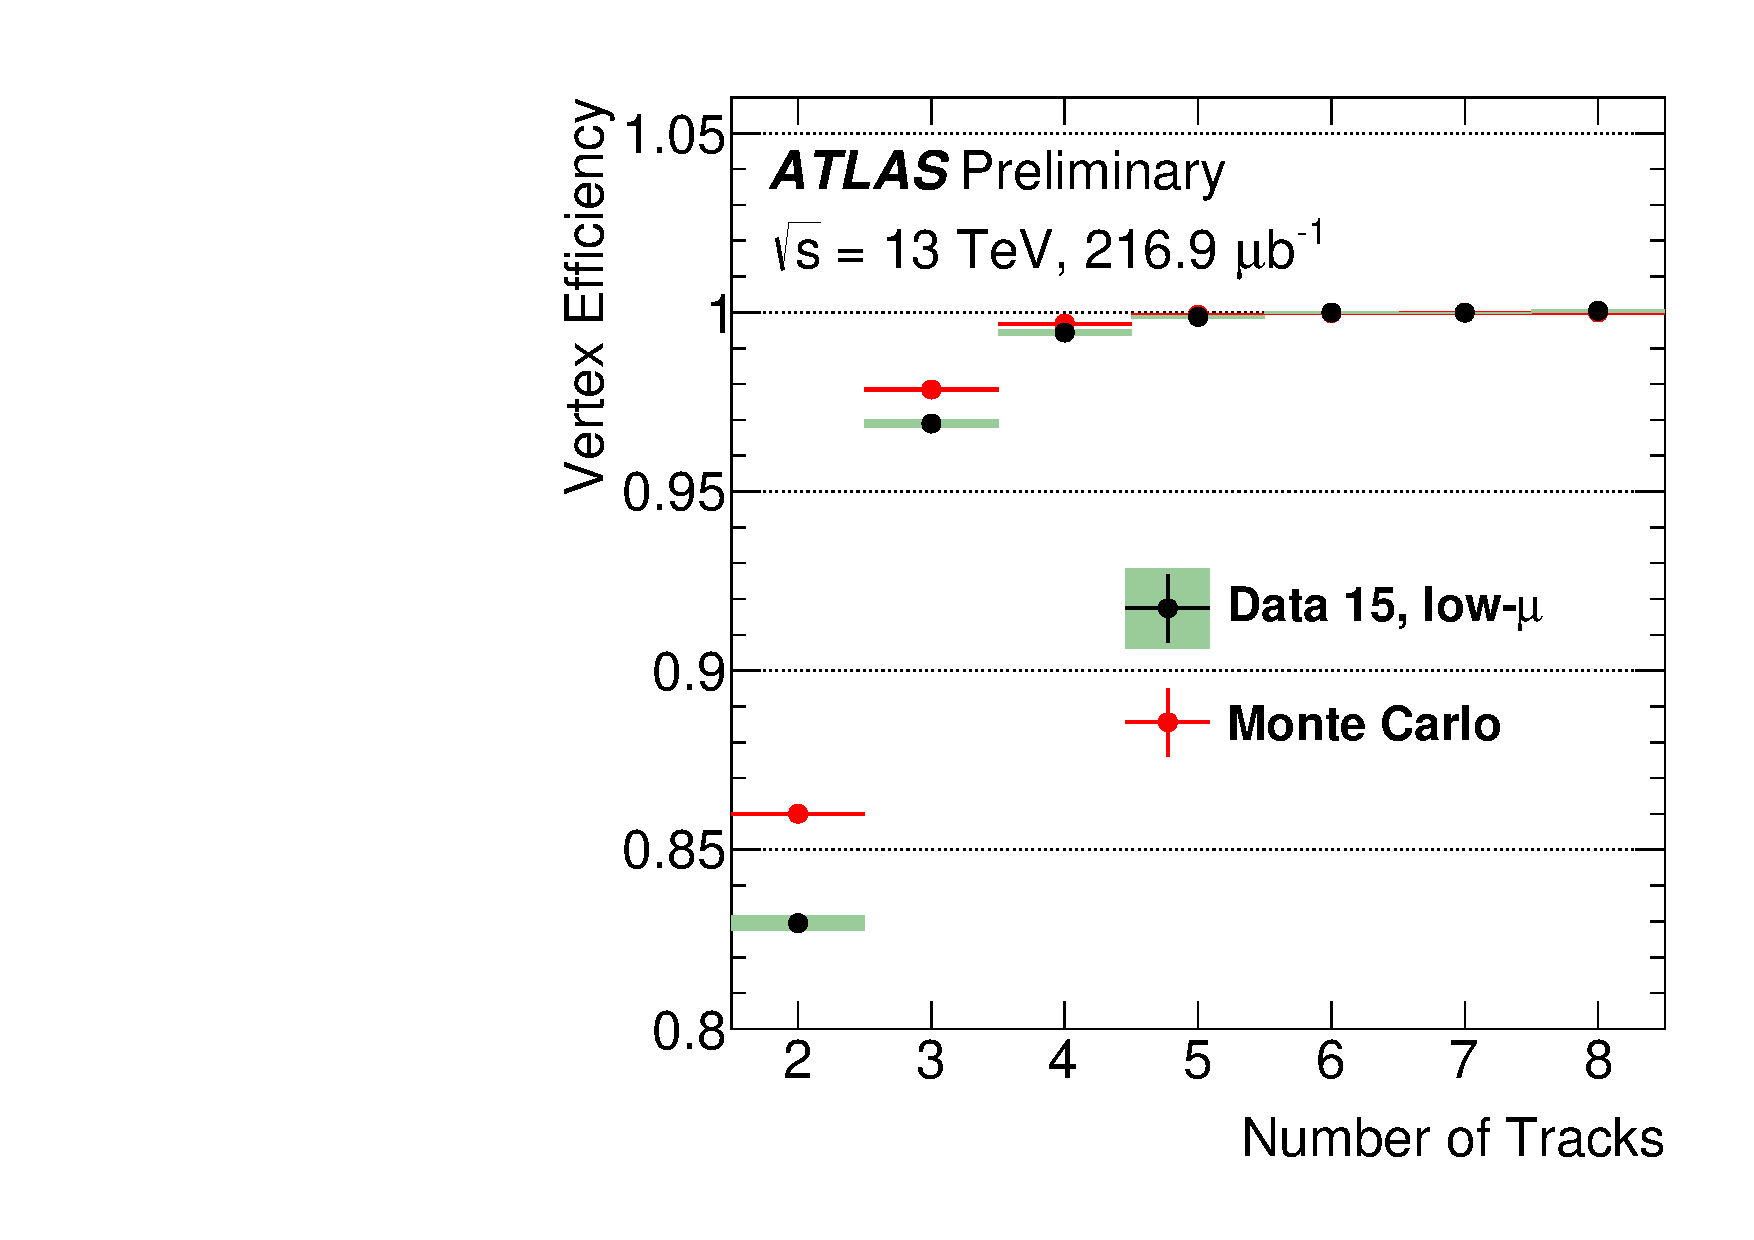
\includegraphics[width=0.55\linewidth]{figures/Reco/TrackingVertex}
\caption{\cite{ATL-PHYS-PUB-2015-026}}
\label{fig:reco-primaryvertexeff}
\end{center}
\end{figure}


